\documentclass{article}
\usepackage{graphicx}
\usepackage[brazilian]{babel}
\usepackage[utf8]{inputenc}
\usepackage[T1]{fontenc}
\usepackage{amsmath}
\usepackage{amssymb}
\usepackage{hyperref}
\setlength{\parindent}{0in}


\begin{document}
	
	\title{Simula IC - MAE0119}
	\author{Daniel Yoshio Hotta – 9922700}
	
	\maketitle	
	
	Enviado termo geral.\\
	
	\textbf {E1.a} 
	\\ \\
	\textit {Resposta:} \\
	
	De fato, o valor de $\epsilon$ independe de $\mu$, basta padronizar $P(|\bar{X} - \mu| \leq \epsilon) = \gamma$ (dividir ambos os lados da desigualdade por $\sqrt{\frac{\sigma^2}{n}}$). Logo:
	
	\begin{center}
		$z_{\gamma/2} = \epsilon / \sqrt{\frac{\sigma^2}{n}}$\\
		$\epsilon = z_{45\%} * \sqrt{\frac{36}{9}}$\\
		$\epsilon = 1.645 * 2$\\
		$\epsilon = 3.29$
    \end{center}
		
	\textbf {E1.b} 
	\\ \\
	\textit {Resposta:} \\	
	
	Comandos utilizados:
	
	\begin{center}
		$x <- rnorm(9, mean = 150, sd = 6)$\\
		$media <- mean (x)$	
		$> ic <- c (med - eps, med + eps)$
	\end{center}
		
	Resultado: $\bar{X} = 156.8323$ (Sim, foi bem atípico, por isso deixei e.e').IC: $[153.5423 160.1223]$.
	
	\begin{center}
		$s <- x - med$\\
		$s <- s * s $\\
		$ s <- sum (s)$\\
		$s <- s / 8$
	\end{center}
		
	Resultado:  $s^2 = 11.50386$. (Realmente, distante da variância, mas a média também estava distante, então...)\\
	
	\textbf {E1.c e d} 
	\\ \\
	\textit {Resposta:} \\	
	
	Código no link : \href{https://github.com/HiimHotta/MAE0119/blob/main/SimulaIC/1c.R}{aqui}.
	
	\begin{figure}[h]
		\caption{Exercício 1c.}
		\centering % para centralizarmos a figura
		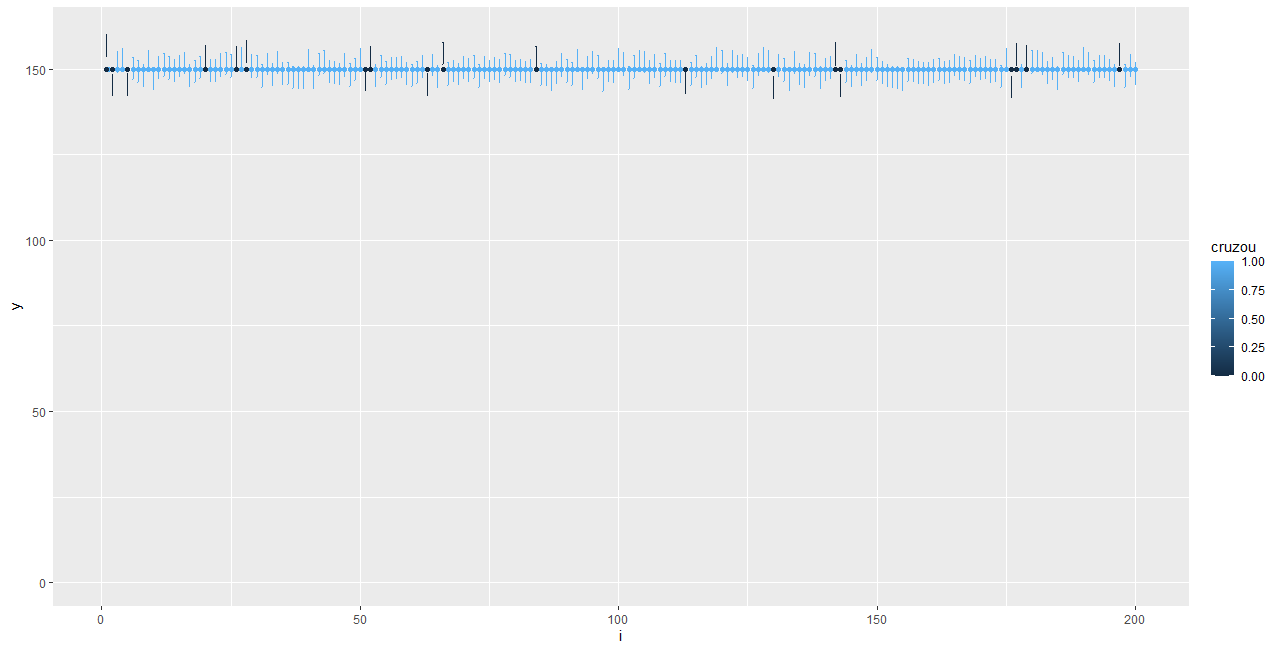
\includegraphics[width=16cm]{ex1c.png} % leia abaixo
		\label{figura:ex3p1}
	\end{figure}

    18/200... Uma quantidade bastante aceitável, já que o correto seria 20/200.
    
    \textbf {E2.a} 
    \\ \\
    \textit {Resposta:} \\	
    
    Código:
    
    \begin{center}
   	    x <- rbinom(1, 100, 0.4)
    \end{center}
    
    Resultado da proporção amostral é 0.41.\\
    
    Calculo pela fórmula do erro amostral:
    
    \begin{center}
    	$\epsilon =  z_{\gamma / 2} * \sqrt{\frac{p (1- p)}{n}}$
    	$\epsilon = 1.96 * \sqrt{\frac{0.24}{100}}$
    	$\epsilon = 0.09601$
    \end{center}

     Logo, o intervalo será: $[0.41 - 0.09601, 0.41 + 0.09601]$\\
     
    \textbf {E2.b e c} 
    \\ \\
    \textit {Resposta:} \\	
    
    Código no link : \href{https://github.com/HiimHotta/MAE0119/blob/main/SimulaIC/2b.R}{aqui}.\\
    
    \begin{figure}[h]
    	\caption{Exercício 2b.}
    	\centering % para centralizarmos a figura
    	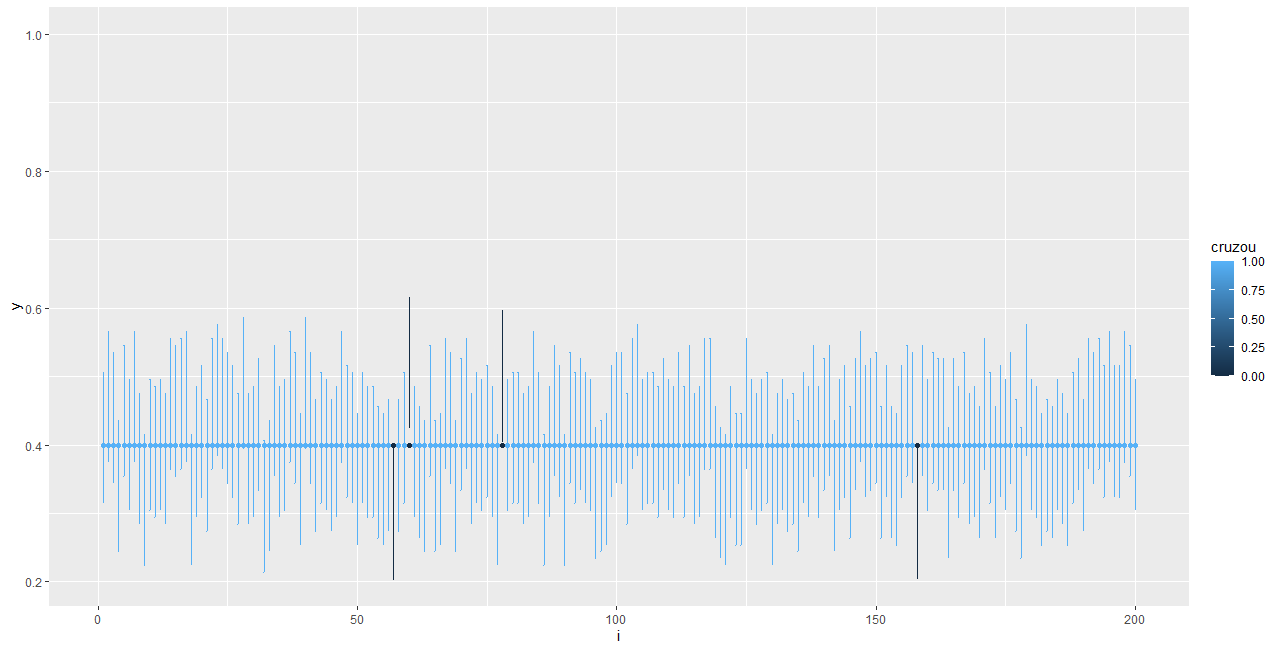
\includegraphics[width=16cm]{2b.png} % leia abaixo
    	\label{figura:ex3p1}
    \end{figure}
    
    4/200 ... Dessa vez, parece que aumentou bem a margem de erro, pois o esperado seria 10/200...
    
	
	\end{document}
